\chapter{Result From Flight Data}\label{ch:FlightResult}

This chapter is divided into three main sections. Firstly, the
algorithm's convergence and consistency was analyzed. Secondly, the
accuracy of the algorithm is examined by comparing to ground truth
data. The third section summarized test results for tuning the
algorithm for better accuracy and efficiency. The forth section
present the advantage of using IMU data. The fifth section outline
the inadequacies of the CC\_EKF\_SLAM algorithm identified.

To test the performance of CC\_EKF\_SLAM algorithm, 4 segments of video
were selected from the test flight video, and 400 frames were
processed in each piece. The filter initialized 40 features at the
first frame, and maintain the tracked features amount at this number
by initializing new features when existing features moved out of FOV.

Since all parameters are tracked in camera frame, their value is 
different when viewed from a fixed point in world frame. Therefore, all 
parameters are converted back to world frame before plotting. 

\section{Convergence and Consistency}

\subsection{Convergence and Tracking}
Among the feature parameters, the feature initialization point were
initialized to the zero which is the origin of the camera centric
coordinate. $\phi$ and $\theta$ were calculated directly from the
feature position on image plane, have high accuracy and don't require
convergence. The only parameter that goes through a converging process
is the features' inverse depth $\rho$, which were initialized to 0.1
for all features. Figure \ref{fltfig:1} shows the $1/\rho$ plot for
video segment1 over 200 frames. The depth estimators went through
rapid changes for several frames after their initialization. Within
approximate 20 frames, most estimtors settles to a stable value. The
estimated features distance ranged from 400 meters to about 1500
meters, confirming the algorithm's capability for estimating features
at great distance. On the other hands, some features take a long time
to settle, while some other never settled, such as 12 and 20.
% is the non and slowly settled feature has any character in its
% pattern? ie. is a line feature, instead of corner? A outlier filter
% should be in place to get rid of the poor features (future work).

\begin{figure}[h]
\centering
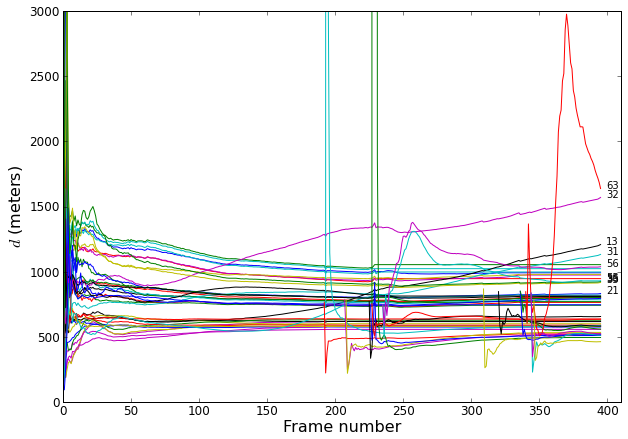
\includegraphics[width=10cm, keepaspectratio=true]{./Figures/fltfig/cut1/Figure10.png}
\caption{Inverse Depth Convergence}
\label{fltfig:1}
\end{figure}

Although the features initialization point $[x_i, y_i, z_i]$, and the
deviation-elevation angle pair $[\phi, \theta]$ did not go through a
converging stage, they do get updated and converted into the new
camera coordinate using the estimated camera motion at every
iteration. As a result, the accuracy of these parameters varies.
Ideally, the coordinates should converge to a fixed value. However,
the plot indicates a variation as the vehicle travels along. Figure
\ref{fltfig:2} shows the tracking of these parameters over the entired
processed frames.
These parameters were stable for about 200 frames. As soon as any
feature was deleted from the filter and new features added, the
parameters of the feature after being converted into world
frame start to drift. In \ref{fltfig:2} the deletion of old feature is
marked by a vertical gray dash line. It shows that the parameters of
the deleted feature start to drift right after that line. The $y_i$
and $z_i$ are most affected. The behavior is caused by the estimated
error in the SUAS localization. In order to compensate the error in
localization(Figure \ref{fltfig:4}), the algorithm made adjustment on the
estimate of  features parameters so that the combinational result
agrees with the measurement. On the other hand, features mapping is
not affected too much by the error in localization. Because their
parameters are transformed in each iteration to the new camera frame
using the estimated SUAS motion which carries the error. As long as
their parameters are updated together with the estimated motion on that
iteration, and transformed back to the world frame using the same
estimated motion, the final result of features location in world frame
is inaffected by the error in the SUAS localization. However, for
feature removed from the filter, their parameters are no longer
updated, therefore revealing the error in SUAS localization. 

\begin{figure}[h]
\centering
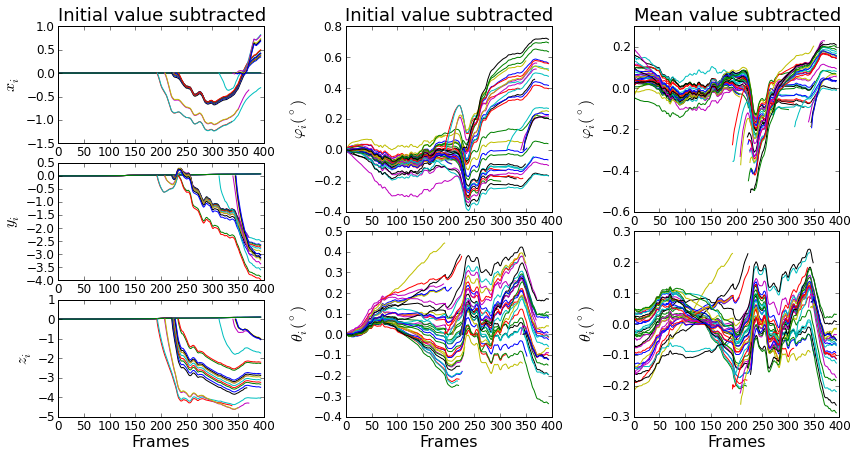
\includegraphics[width=12cm, keepaspectratio=true]
{./Figures/fltfig/cut1/Figure20.png}
\caption{Feature parameters tracking}
\label{fltfig:2}
\end{figure}

\subsection{Consistency Analysis}
A EKF system becomes inconsistent when the variance of state vector
element becomes too small and forbid an effective update. In addition,
the uncertainty of the SUAS position should increases as it move away
from the origin. To examine the consistency of the CC\_EKF\_SLAM
algorithm, the variance of all state vectors for all procesed frames
were extracted and plotted in figure \ref{fltfig:3}. The two plots on
the left shows the variance of world frame position and orientation in
camera frame. The three plots on the right show the variance of
feature parameters. The variance of world frame position increases
with iterations. On the other hand, world frame orientation decreases
with iterations. Especially the orientation in Y and Z axis remain
below 5e-7 for the most time. For feature parameters, all variance
decreases with iterations, and their value is very small. 
\begin{figure}[h]
\centering
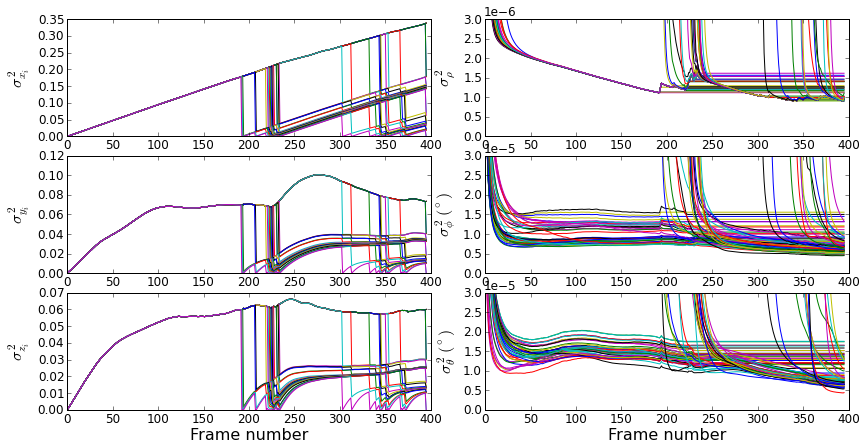
\includegraphics[width=12cm, keepaspectratio=true]
{./Figures/fltfig/cut1/Figure40.png}
\caption{State vector variance}
\label{fltfig:3}
\end{figure}

To see how variance affect the correction the filtered made on the
state vector, the correction applied each iteration were plotted ni
figure \ref{fltfig:4}. The $1^{st}$ column shows the correction on
world frame position in camera frame. The $2^{nd}$ column shows the
correction on feature initialization coordinate in camera frame. The
$3^{rd}$ column shows the correction on features parameters $\rho$,
$\phi$ and $\theta$. It can be observed that world frame position on Y
and Z component receive more correction than the X component, despite
their variance is smaller than the X axis. Similarly, feature
parameter $\theta$ and $\phi$ receive more correction than $\rho$
despite their variance is smaller than the variance of $\rho$.
Secondly, there is a strong inverse correlation between the Y and Z
component of feature initialization position and the world frame
position on Y and Z axis. Similarly, $\phi$ is correlated to world
frame position Z component, $\theta$ is correlated to the world frame
position Y component. Since the features initialization coordinate has
high correlation with the world frame Y and Z position, the main
contributor all the drift comes from the world frame position
correction. Figure \ref{fltfig:5} shows the Kalman Gain over the 5
iteration for the first 35 elements in the state vector, which include
world frame parameters, SUAS motion parameters, and parameters for the
first 4 features. At $1^{st}$ iteration, the high gain is on the
feature parameter $\rho$. Starting from the $2^{nd}$ iteration, more
and more weight goes into the Y and Z component of world frame
position, as well as the Y and Z component of features initialization
position. Although the variance of these two parameters is small, it
is possible that the linearization of the measurement model increased
the correction gain on these parameter. This issue requires further
digging, and will be analyze as a future work.  

\begin{figure}[h]
\centering
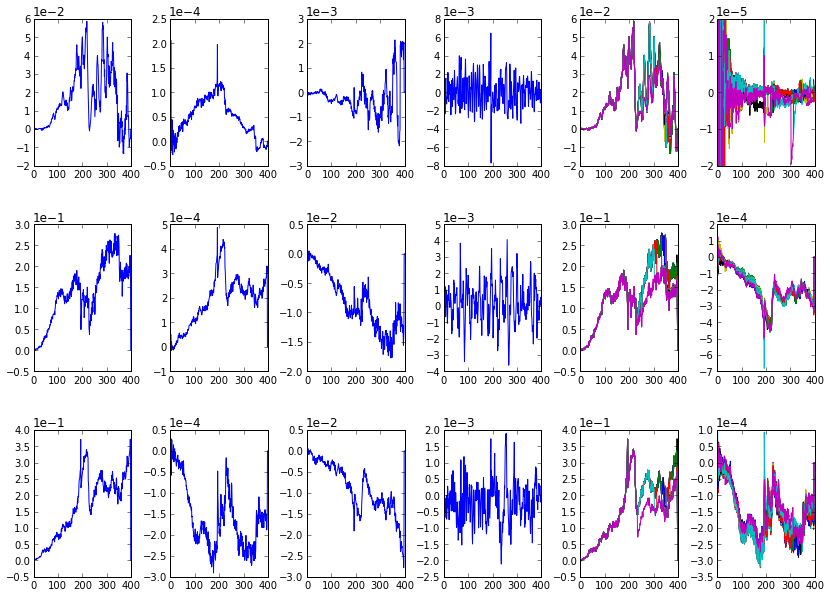
\includegraphics[width=12cm, keepaspectratio=true]
{./Figures/fltfig/cut1/Figure112.png}
\caption{State Vector Corrections}
\label{fltfig:4}
\end{figure}

\begin{figure}[h]
\centering
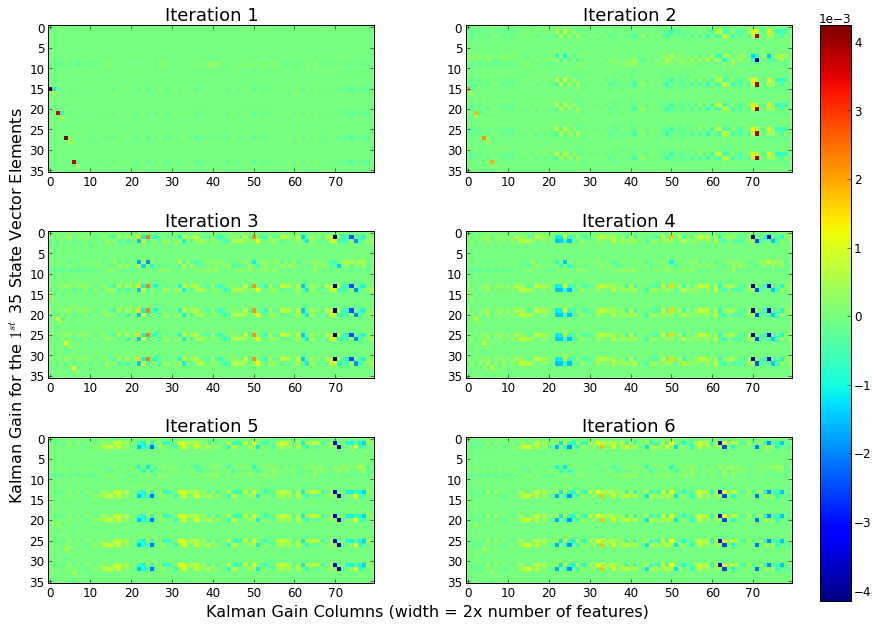
\includegraphics[width=14cm, keepaspectratio=true]
{./Figures/fltfig/cut1/Figure113.png}
\caption{Kalman Gain Matrix for the first 35 State Vector Elements}
\label{fltfig:5}
\end{figure}

In summary of the consistency analysis, the filter has not moved into
inconsistent state at 400 iterations. However, the variance of
parameters does decrease at each iteration that it is only a matter of
time that the filter will become inconsistent. Therefore, the filter
will require a reset procedure to 

\begin{enumerate}
  \item Resync the SUAS location with GPS. 
  \item Reset its covariance matrix. 
\end{enumerate}

\noindent for any large area operation. 

\section{Accuracy}
\subsection{SUAS Localization}

The SUAS location and orientation were verified in UTM coordinate.
Ground truth data comes from the GPS for position, and magnetometer
for orientation. The GPS positioning can generally achieve 7.8 meters
in accuracy \cite{_gps_????}. For orientation, accuracy on the
datasheet specified $0.1^{\circ}$ for roll and pitch, and
$0.5^{\circ}$ for heading. Figure \ref{fltfig:6} shows the estimated
SUAS position and orientation, ground truth data, and the error. From
the comparison, X position error reached 20m maximum, while Y and Z
position error is bigger, reaching 50 meter and 30 meters respectly.
For orientation, the estimated value agrees with the ground truth
pattern, with maximum error within 0.02 rad or $1.15^{\circ}$.
Although the error of pitch is biased to the negative side, and error
of heading is biased to the positive side. there was not sign of error
diverging within the 400 frames processed.

\begin{figure}[h]
\centering
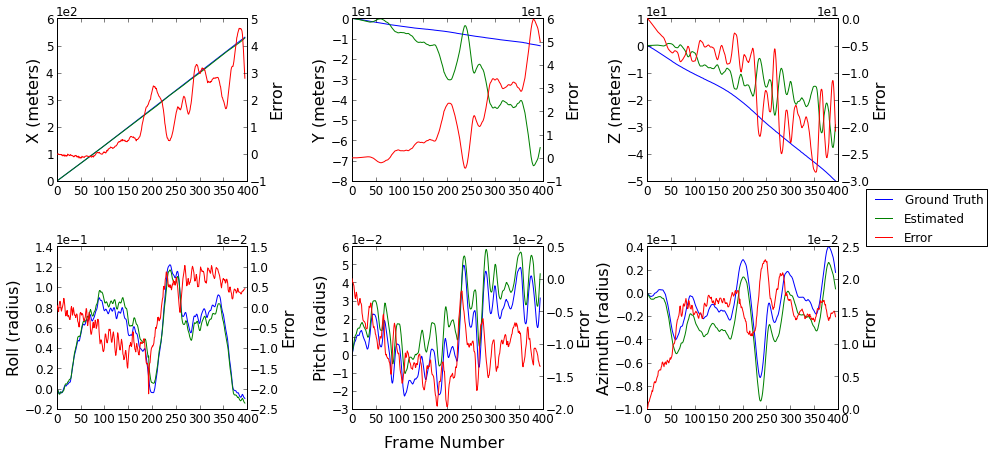
\includegraphics[width=12cm, keepaspectratio=true]
{./Figures/fltfig/cut1/Figure30.png}
\caption{SUAS position and orientation}
\label{fltfig:6}
\end{figure}

\subsection{Features Mapping}

Although raw ground truth data for the terrain was downloaded from
\cite{_cgiar-csi_????} CGIAR-CSI website, making data correspondence
with the estimated feature is non-trival for natual scene where it
lacks of signature landmark sucn as building corners. From the
experience of analyzing simulation data (chapter 6), the initialized
feature deviation and elevation angle $\phi$ and $\theta$ agrees very
well to the ground truth value. In addition, feature initialization
position is set to $[0, 0, 0]$ in camera frame, therefore carris no
error. Therefore, the following procedure are used the find the
corresponding ground truth location for any estimated feature. 

\begin{enumerate}
  \item The frame number at which feature was initialized was
  identified, and ground truth location of the SUAS at that frame was
  recorded.
  \item Shift DEM to the initialization point using the SUAS ground
  truth location recorded
  \item Align the feature deviation $\theta$ and elevation $\phi$ angle to UTM frame.
  (These angles were recorded in camera frame)
  \item Create a vertical plane using $\theta$ and slice the DEM to
  form a 1D elevation plot (Figure \ref{fltfig:7} blue line)
  \item Create a line using $\phi$ and intersect the 1D elevation plot
  (Figure \ref{fltfig:7} green line). The $1^{st}$ intersection point
  is used as ground truth feature location.
\end{enumerate}

\begin{figure}[h]
\centering
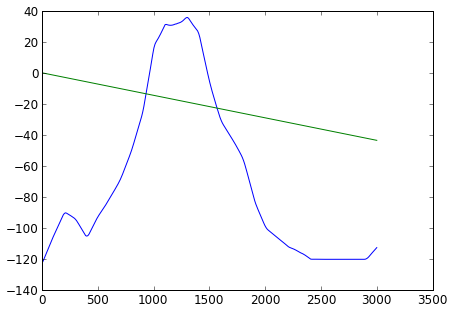
\includegraphics[width=12cm, keepaspectratio=true]
{./Figures/fltfig/cut1/intersect0_0.png}
\caption{Feature position error}
\label{fltfig:7}
\end{figure}

By comparing to the ground truth feature location extracted using the
method describe above, figure \ref{fltfig:8} shows the feature
position error convergence plot in world frame. Feature locations are
compared in world frame for the ease of corresponding the estimated
features and terrain plot with the video by eye. The error convergence
is plotted in figure \ref{fltfig:8} top left. X component (along which
axis the SUAS is traveling) of feature position converge to near zero
in general with maximum error less than 120m for the converged
features. Y component shows a clear offset for features not
initialized at first frame. This behavior is similar to what's seen in
the simulation analysis \ref{sec:featureMotion} where offset in features
position estimates are caused by drift in SUAS localization
estimation. In this case, the features position were converted into
world frame using the estimated SUAS position, while the ground
truth feature position are found using the ground truth SUAS position,
which is different than the estimated. Therefore the offset error can
be seen. Z component does not show such offset, but some features' Z
component position drift away after new features were added into the
filter. This drift could be related to the drift in estimates of angle
$\phi$ (figure \ref{fltfig:2}).

\begin{figure}[h]
\centering
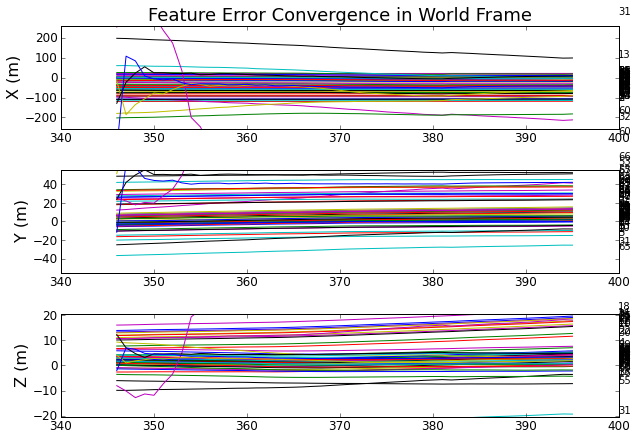
\includegraphics[width=7cm, keepaspectratio=true]
{./Figures/fltfig/cut1/Figure50.png}
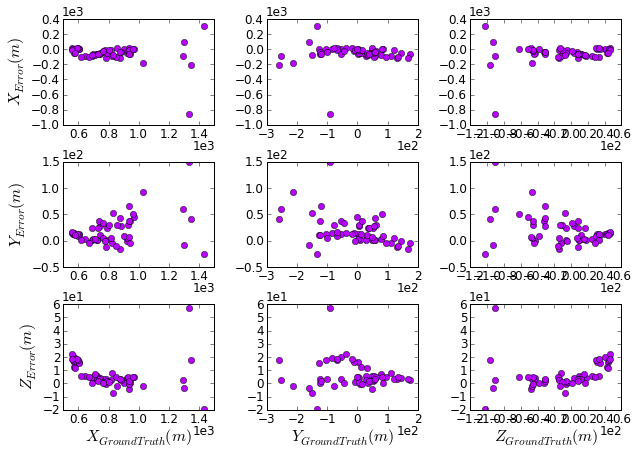
\includegraphics[width=7cm, keepaspectratio=true]
{./Figures/fltfig/cut1/Figure80.png}
\caption{Left: , right: }
\label{fltfig:8}
\end{figure}

Plotting the actual estimated and ground truth features position
reveals relation between the error and the feature's position. Figure
\ref{fltfig:9} bottom plots the feature positions and error at frame
398. First on X axis, the biggest error occur on feature number 65
which is initialized pretty late in the sequence, and has not
converged properly. On Y axis, the position plot also shows feature
number higher than 40 carries an offset error. In addition, the
average error is increasing as feature number gets bigger, which
indicate the further the feature initialization point is from the
world origin, the bigger this offset error will me. On Z axis, besids
the feature 65 carries a big error, features with ground truth Z
position bigger than 25 generally has an error of 15-20 meters. If the
error are plotted against the ground truth position (figure
\ref{fltfig:8} right), it can be seen that these features all
located within 600 meters to the camera. 

\begin{figure}[h]
\centering
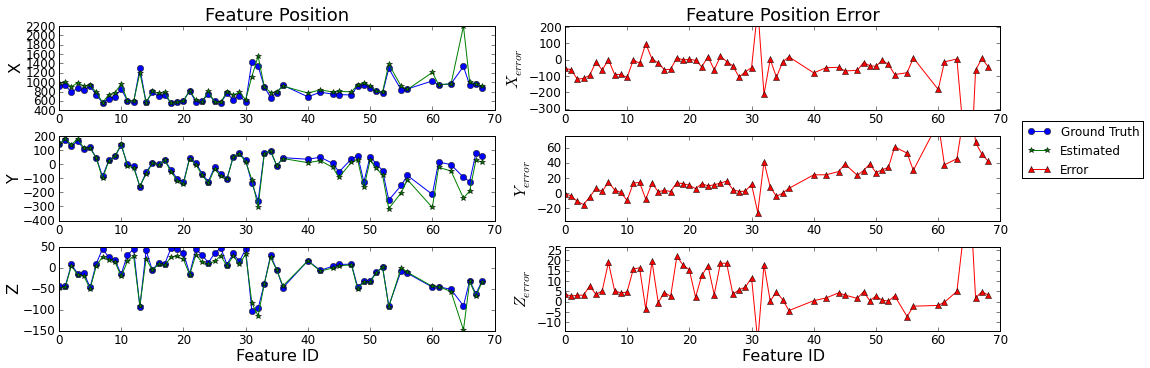
\includegraphics[width=14cm, keepaspectratio=true]
{./Figures/fltfig/cut1/Figure60.png}
\caption{Feature position and error. Left: , right: }
\label{fltfig:9}
\end{figure}

Using the estimated feature position, a terrain map can be generated.
Figure \ref{fltfig:10} shows the terrain map generated from the
feature position analyzed above. On the right, the ground truth DEM is
also shown for comparison. 

\begin{figure}[h]
\centering
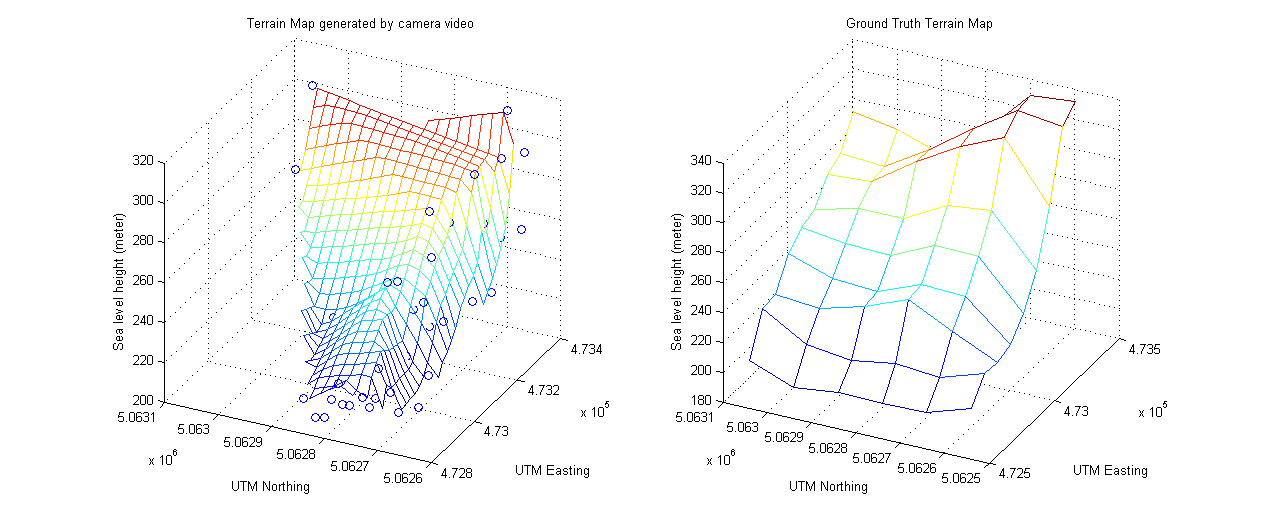
\includegraphics[width=14cm, keepaspectratio=true]
{./Figures/fltfig/cut1/terrain/terrain_map_cmp.png}
\caption{Terrain map. Left: estimated, right: ground truth }
\label{fltfig:10}
\end{figure}

\section{Compare to Visually Corresponded Feature}
Because it is hard to correspond feature extracted from video to the
actual data on DEM, a second piece of video was processed with
man-made structure in the scene so that feature correspondence can be
made manually. Figure \ref{fltfig:11} shows a zoomed in view of the
features extracted by the CC\_EKF\_SLAM. All features are located at
the bottom left corner of the image. Figure \ref{fltfig:12} shows the
common features found manually on the satalite imaging on Google Earth
\cite{}.

\begin{figure}[h]
\centering
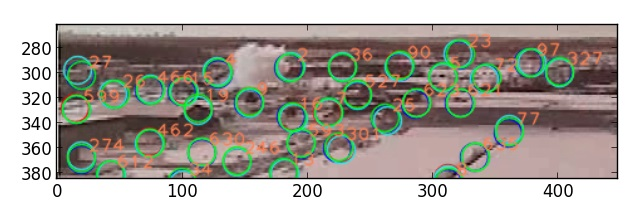
\includegraphics[width=10cm, keepaspectratio=true]
{./Figures/fltfig/airport/frame398_features.jpg}
\caption{Feature identified by algorithm }
\label{fltfig:11}
\end{figure}

\begin{figure}[h]
\centering
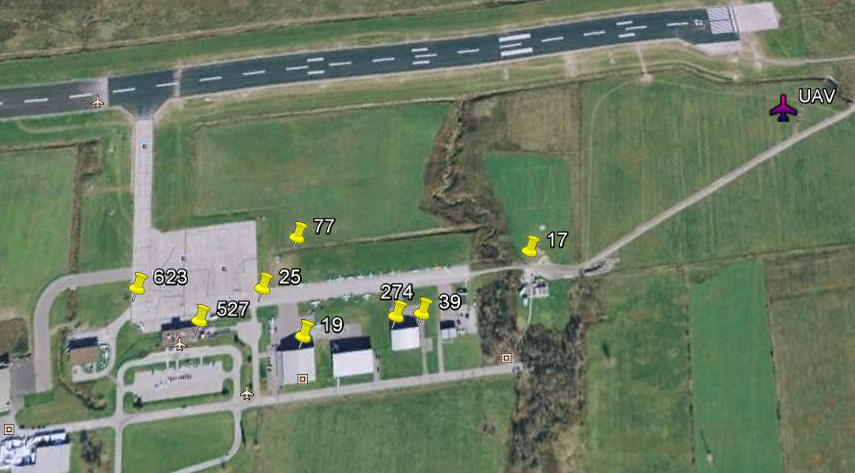
\includegraphics[width=13cm, keepaspectratio=true]
{./Figures/fltfig/airport/uav_and_identified_landmark.png}
\caption{Common features idetified manually on Google Earth }
\label{fltfig:12}
\end{figure}
\FloatBarrier

The SUAS position and orientation were compared to onboard GPS and INS
recording, and the result are plotted in figure \ref{fltfig:13} and
figure \ref{fltfig:14}. Similar to the natual scene video, SUAS
location is more accurate on X, and shows more drift on Y and Z
coordinate. The drift become significant when frame number exceeds
200. However, with the SUAS decending, drift on Z is less than when it
is ascending. For orientation error, roll and pitch error oscillate
around zero, but azimuth error drift away as frame number increases. 

\begin{figure}[h]
\centering
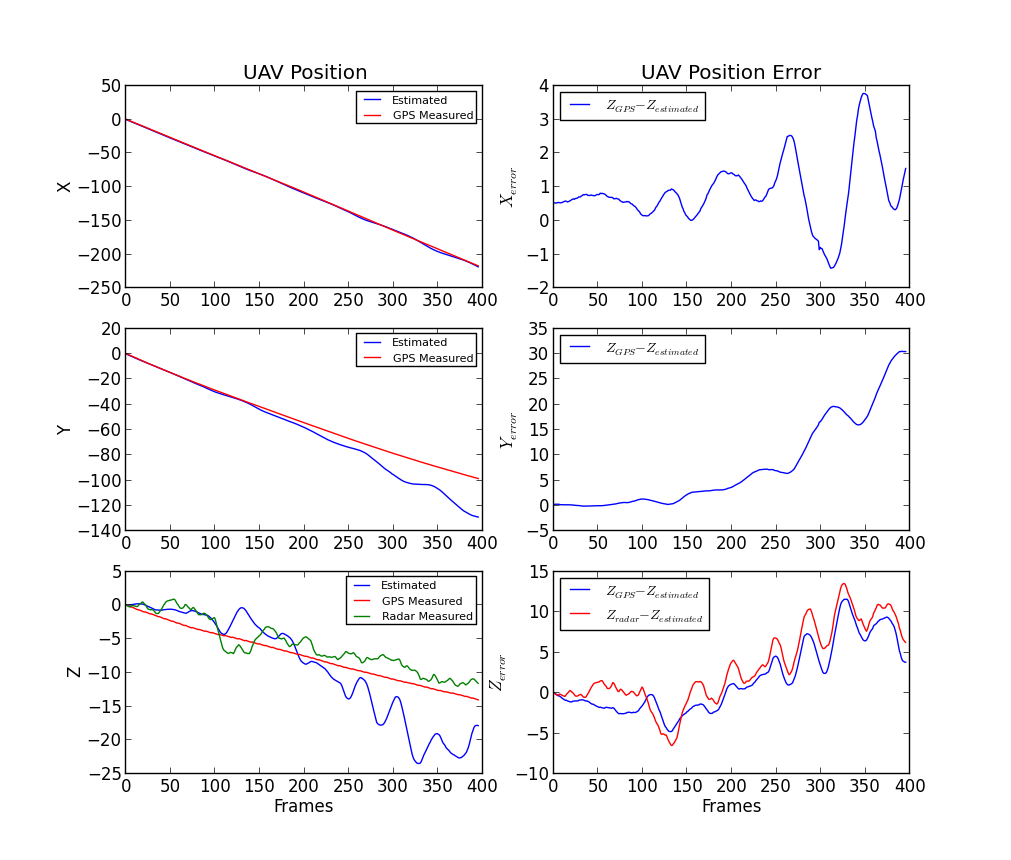
\includegraphics[width=10cm, keepaspectratio=true]
{./Figures/fltfig/airport/UAV_position_and_error.png}
\caption{SUAS position accuracy compared to GPS}
\label{fltfig:13}
\end{figure}

\begin{figure}[h]
\centering
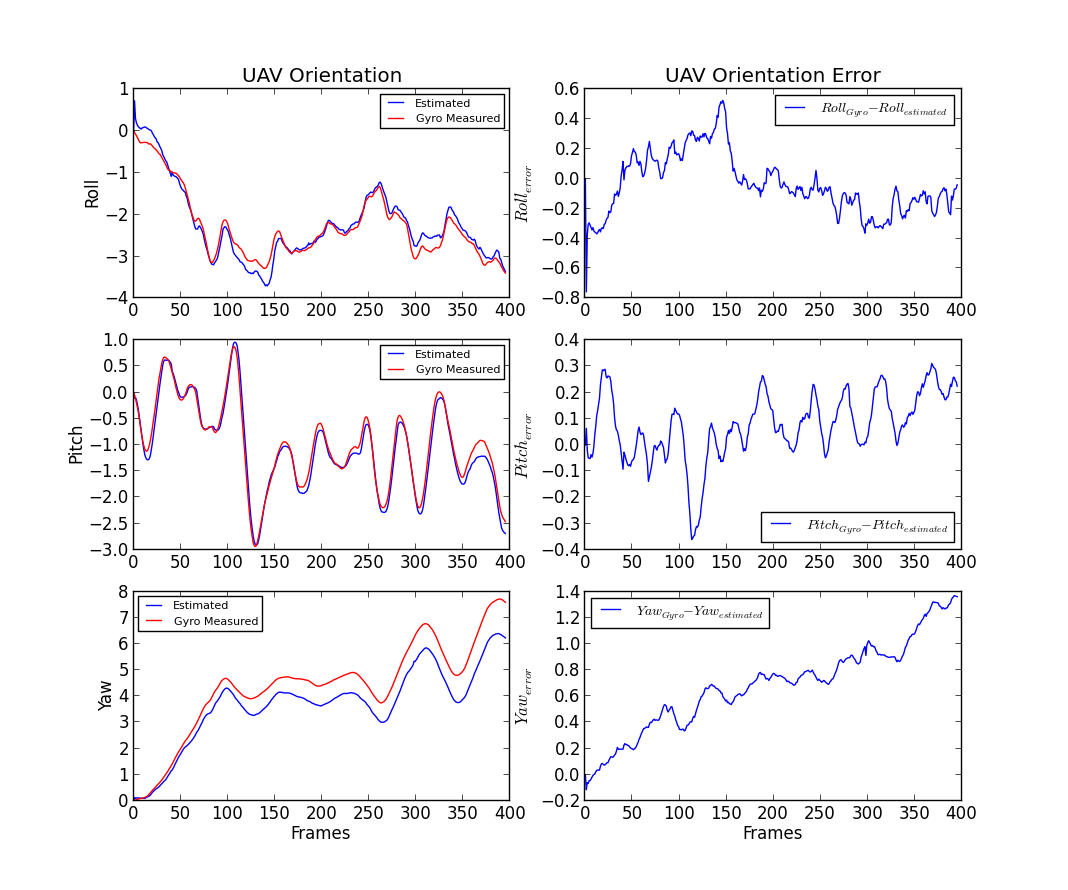
\includegraphics[width=10cm, keepaspectratio=true]
{./Figures/fltfig/airport/UAV_orientation_and_error.png}
\caption{SUAS orientation accuracy compared to ??}
\label{fltfig:14}
\end{figure}
\FloatBarrier

Figure \ref{fltfig:15} shows the features location in X and Y axis.
The google earth map provide a very rough elevation data, and was not
used. The ground truth X and Y coordinate of the features were
measured on Google Earth in GPS coordinates and converted into UTM.
This plot shows a clear offset error between the ground truth and the
estimated. X axis coordinate has a mean offset is about 100 meters,
and Y axis coordinate has a offset of about 130m. Since all features
are located in the bottom left corner of the FOV, it is possible that
lens distortion plays a important part in contributing to these error. 


\begin{figure}[h]
\centering
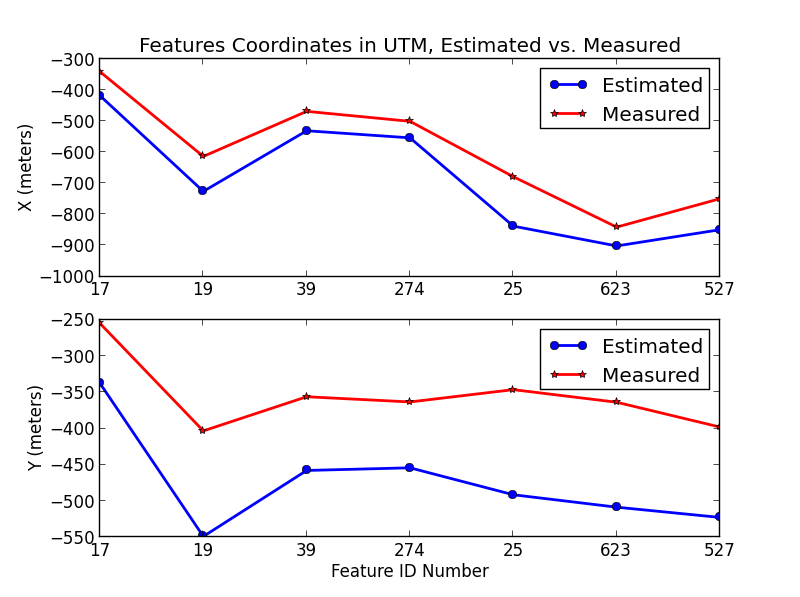
\includegraphics[width=13cm, keepaspectratio=true]
{./Figures/fltfig/airport/Feature_plot_(x,y).png}
\caption{Feature error on X and Y axis. }
\label{fltfig:15}
\end{figure}

%%% Local Variables:
%%% mode: latex
%%% TeX-master: "thesis"
%%% End:
